%%____________________________________________________________________________||

\section{Validation with \texorpdfstring{\gj}{gamma+jets} sample}
\label{app:gjets}

\subsection{Estimate of non-prompt contribution in \texorpdfstring{\gj}{gamma+jets} events}
\label{sec:photon-purity}

The contribution from non-prompt (``fake'') photons in the \gj control 
region~(\ref{sec:photoncontrolSelection}) is expected to be small after
the tight ID and acceptance requirements~(\ref{sec:photon-id}). 
Nevertheless a data-driven estimation of the non-prompt photons is
employed. 

In the previous version of the analysis, the QCD Monte Carlo samples
were reweighted using data$/$MC corrections derived in a fake-enriched
$\sigma_{i\eta i\eta}$ sideband as a function of photon \Pt. This
required subtracting the prompt photon contribution in the sideband
using simulation, which although small for the most part, was quite
sizeable in analysis bins with large \njet and \HT (up to 50-70\%).
Therefore this method was not sufficiently robust, and an alternative
method (a ``template fit'' method) has been employed as described in
the following.
%Both methods agree within statistical uncertainties

In this method, a template maximum likelihood fit is performed to the
charged hadron isolation distribution of the photons in data. This
allows both the fake and prompt components to be constrained
simultaneously. The templates for the non-prompt photons are either
taken from simulation or are extracted from the fake-enriched
$\sigma_{i\eta i\eta}$ sideband (0.011 $< \sigma_{i\eta i\eta} <$
0.02).  The templates for the prompt photons is obtained via the
``random cone'' method \cite{random-cone}, in which the charged hadron
isolation distribution is constructed by randomising the direction of
prompt photons in data and recomputing their isolation value.

The fit is performed over a 0-10~GeV range in isolation, and the
resulting best fit value for the fraction of fakes is used to compute
an estimate of the non-prompt yield in the nominal \gj control region
(chHadIso $<$ 0.202). The fit is performed twice, using templates for
the non-prompt component from simulation and from the $\sigma_{i\eta
  i\eta}$ sideband. The final value for the yield is taken as the
average of those obtained using these two schemes. The difference
halved is taken as a systematic uncertainty.
% fake templates integrated over HT

Two example fits are shown in Fig.~\ref{fig:photonTemplateFits}. The
relative conribution of non-prompt photons in the \gj control region
is shown as a function of (\njet,\HT) in
Fig.~\ref{fig:photon-purities}.  The study confirms a high photon
purity for the selection applied in this analysis, with a typical fake
photon component between 1-5\%.

\begin{figure}[h!]
  \centering
  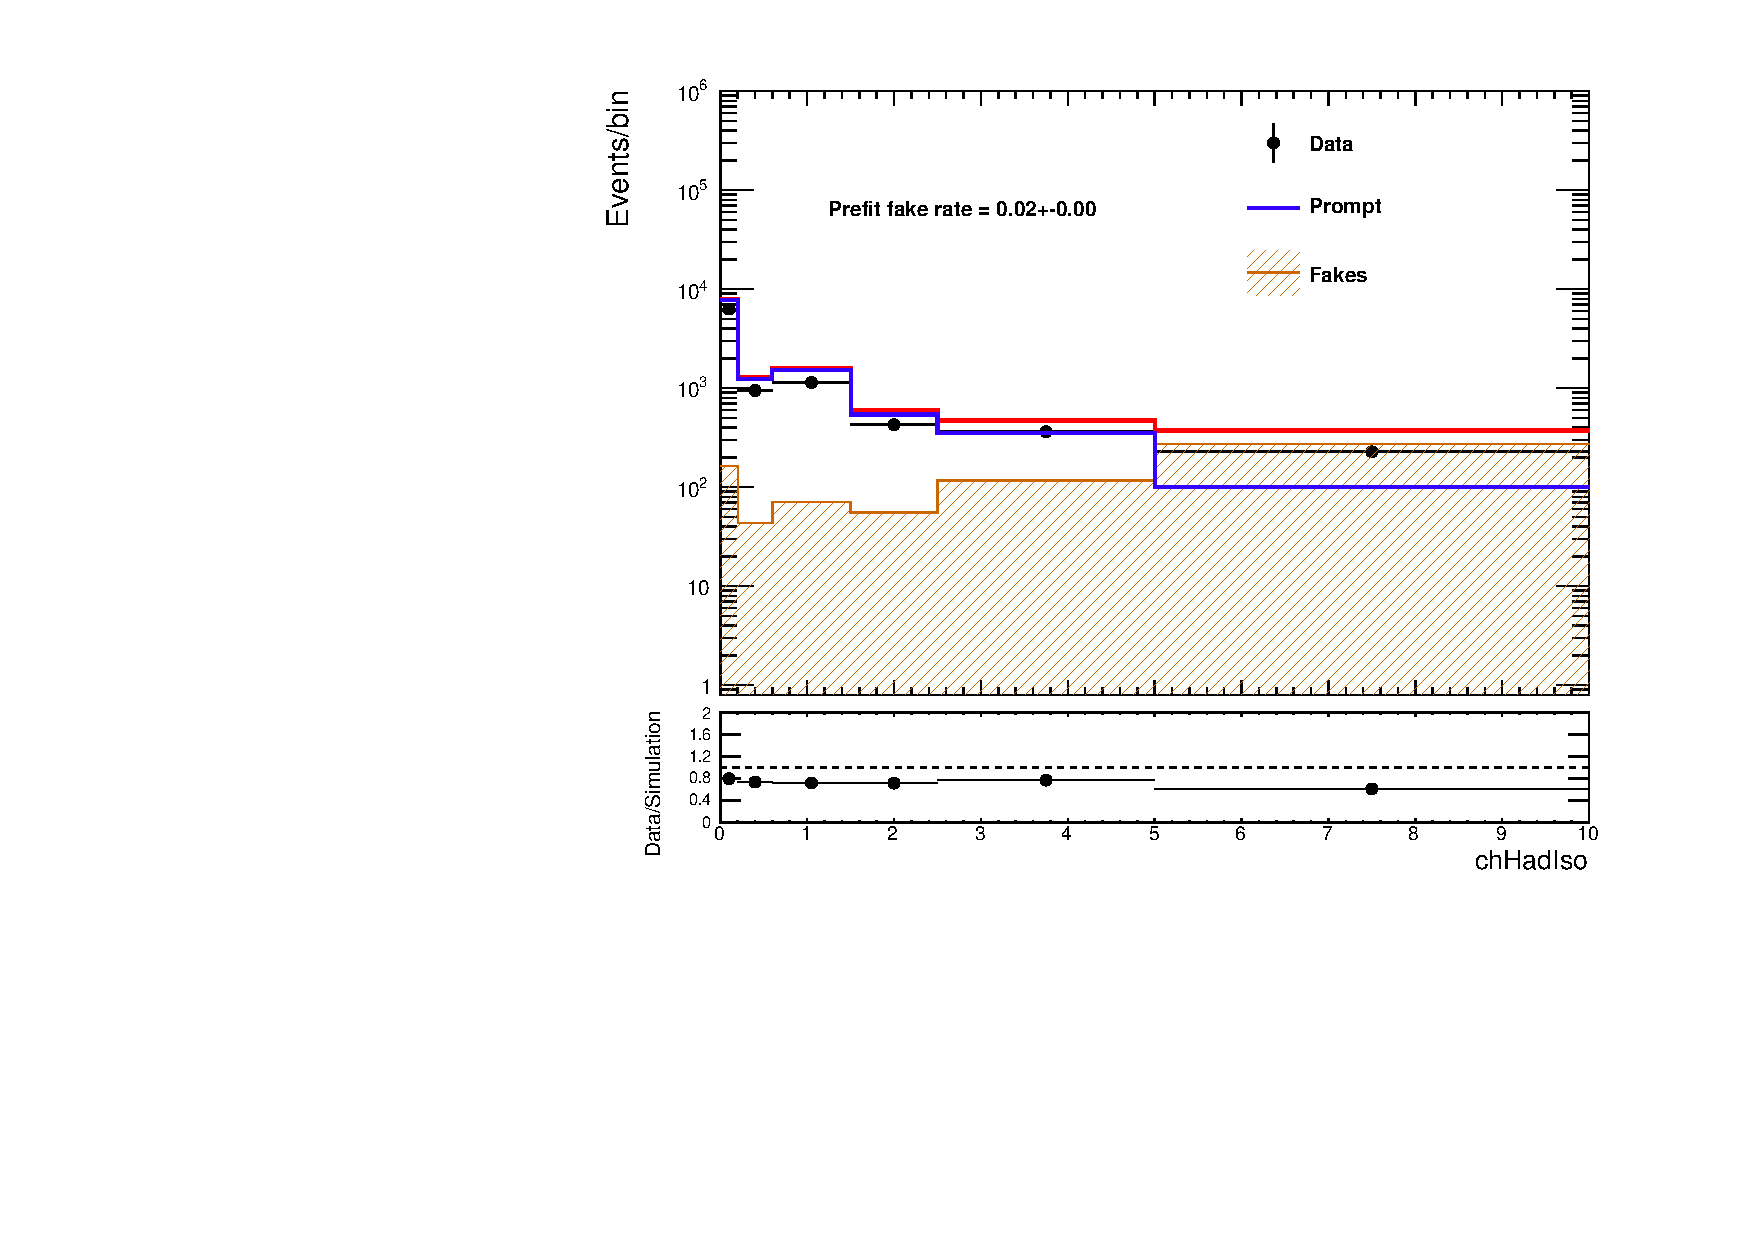
\includegraphics[width=0.45\textwidth]{figures/photonpurity/fakeFit_eq2j_600_prefit} ~
  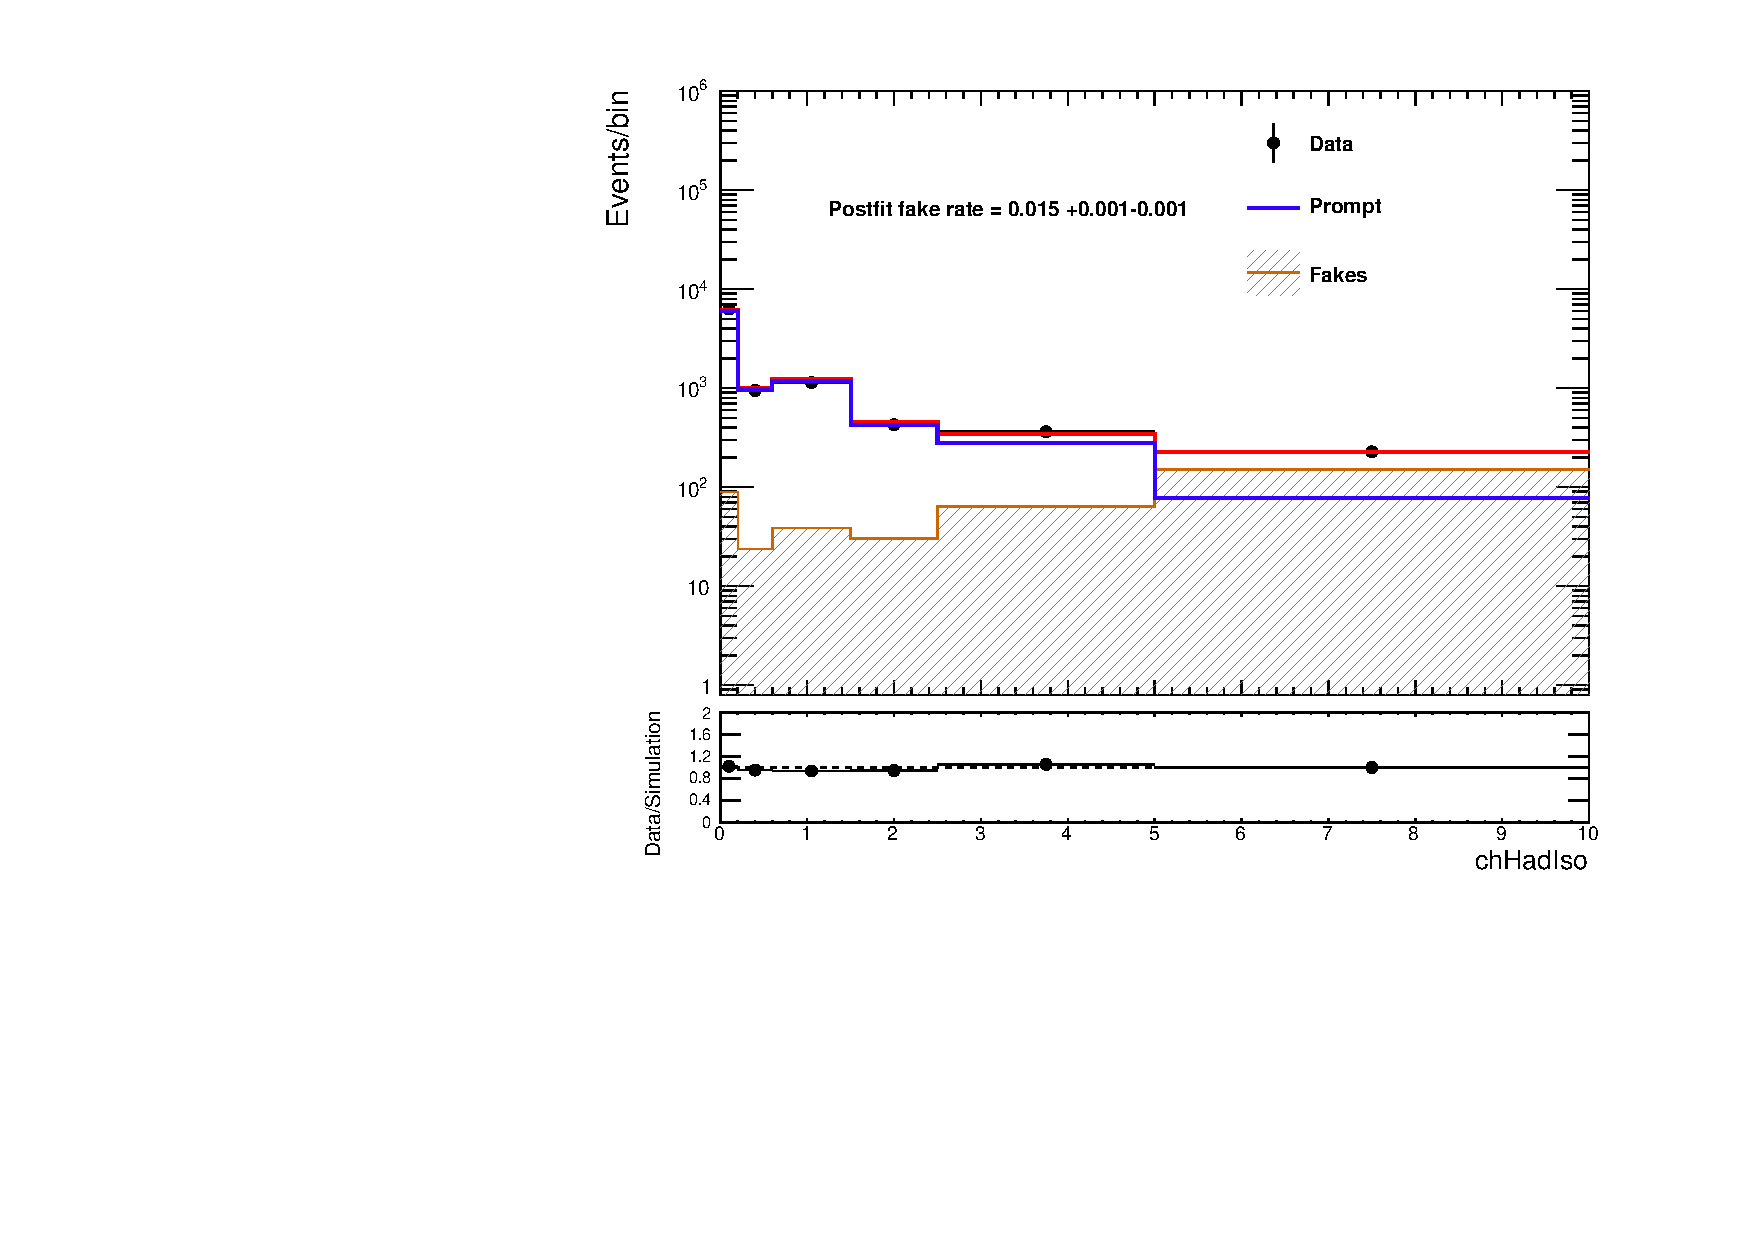
\includegraphics[width=0.45\textwidth]{figures/photonpurity/fakeFit_eq2j_600_postfit} \\
  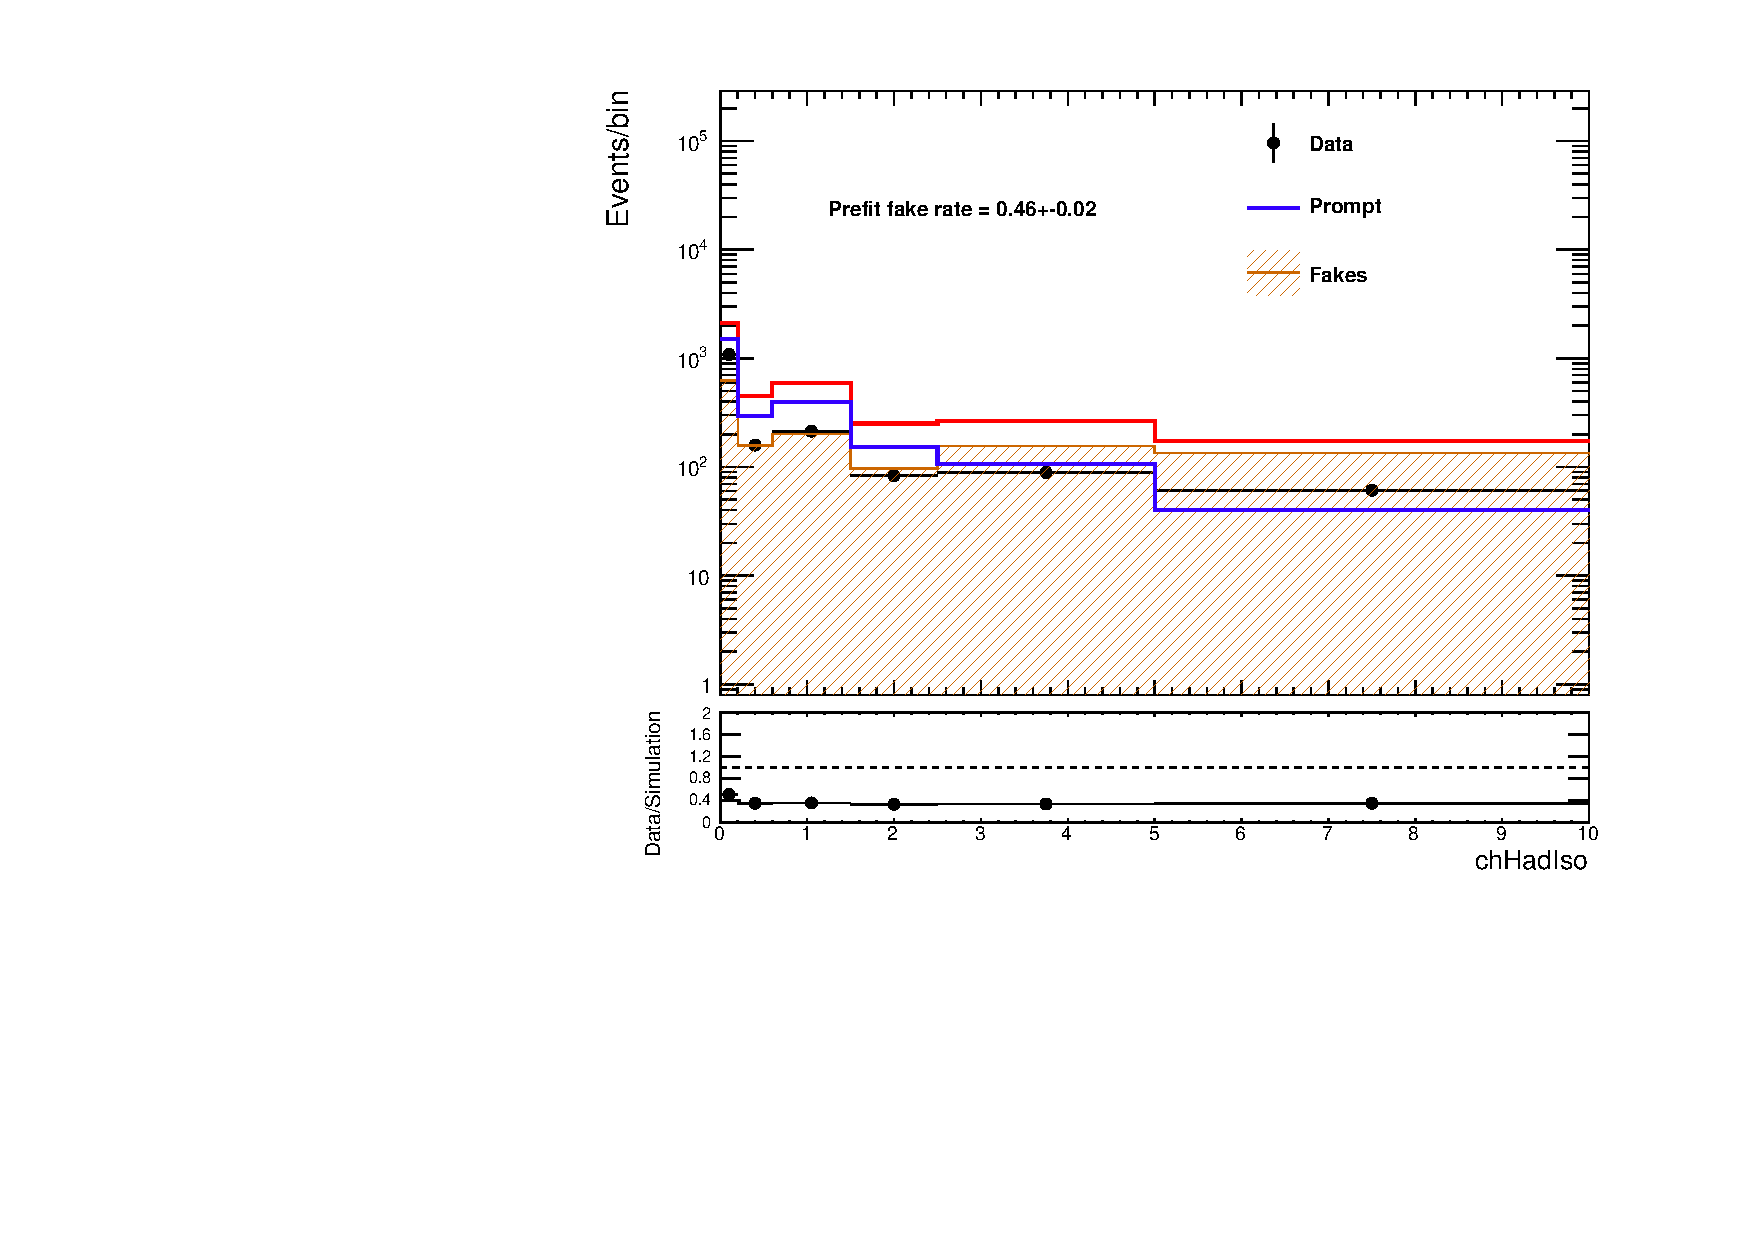
\includegraphics[width=0.45\textwidth]{figures/photonpurity/fakeFit_ge5j_900_prefit} ~
  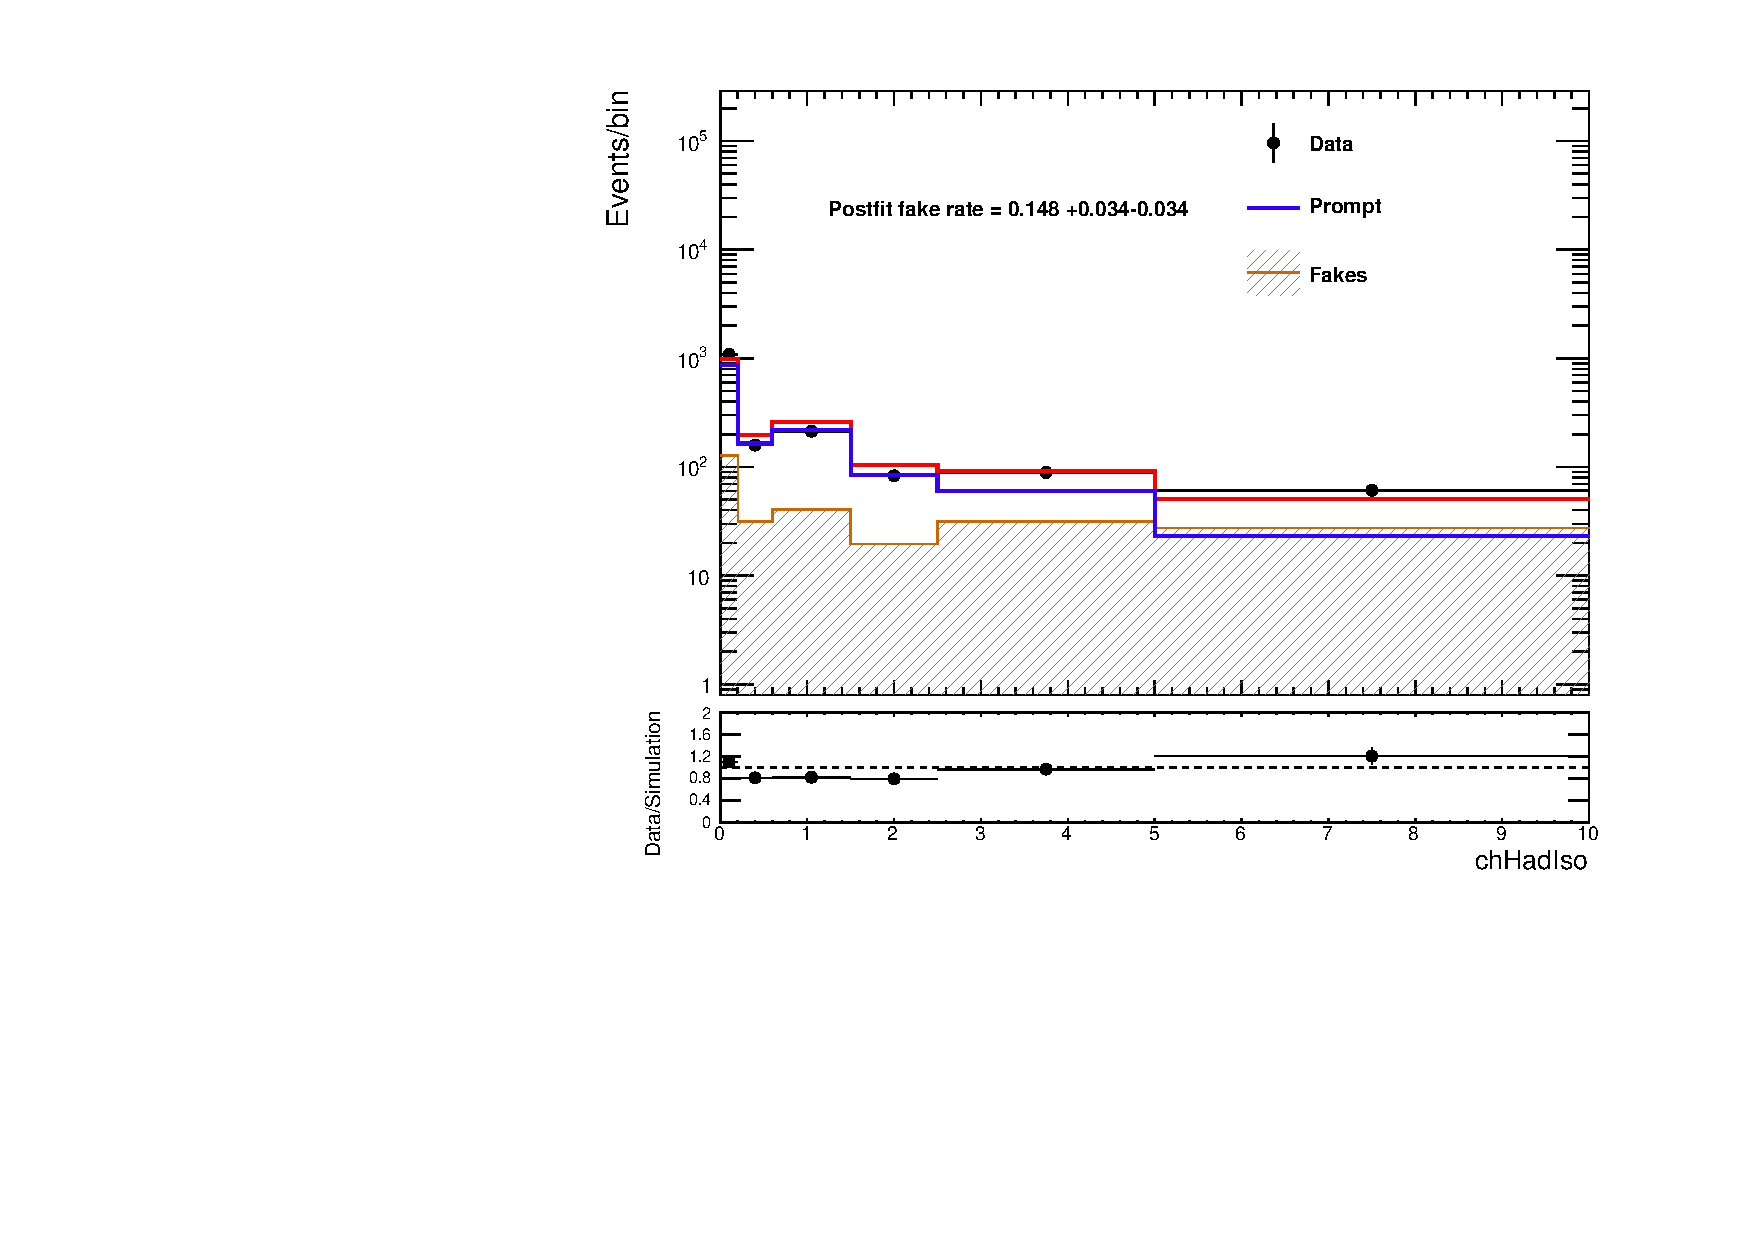
\includegraphics[width=0.45\textwidth]{figures/photonpurity/fakeFit_ge5j_900_postfit}
  \caption{\label{fig:photonTemplateFits} 
  Example prefit (left) and postfit (right) charged hadron isolation
  distributions in the (\njet$=2$, \HT$=600-900$) (top) and 
  (\njet$=5$, \HT$=900-1200$) (bottom) bins.}
\end{figure}


\begin{figure}[h!]
  \centering
  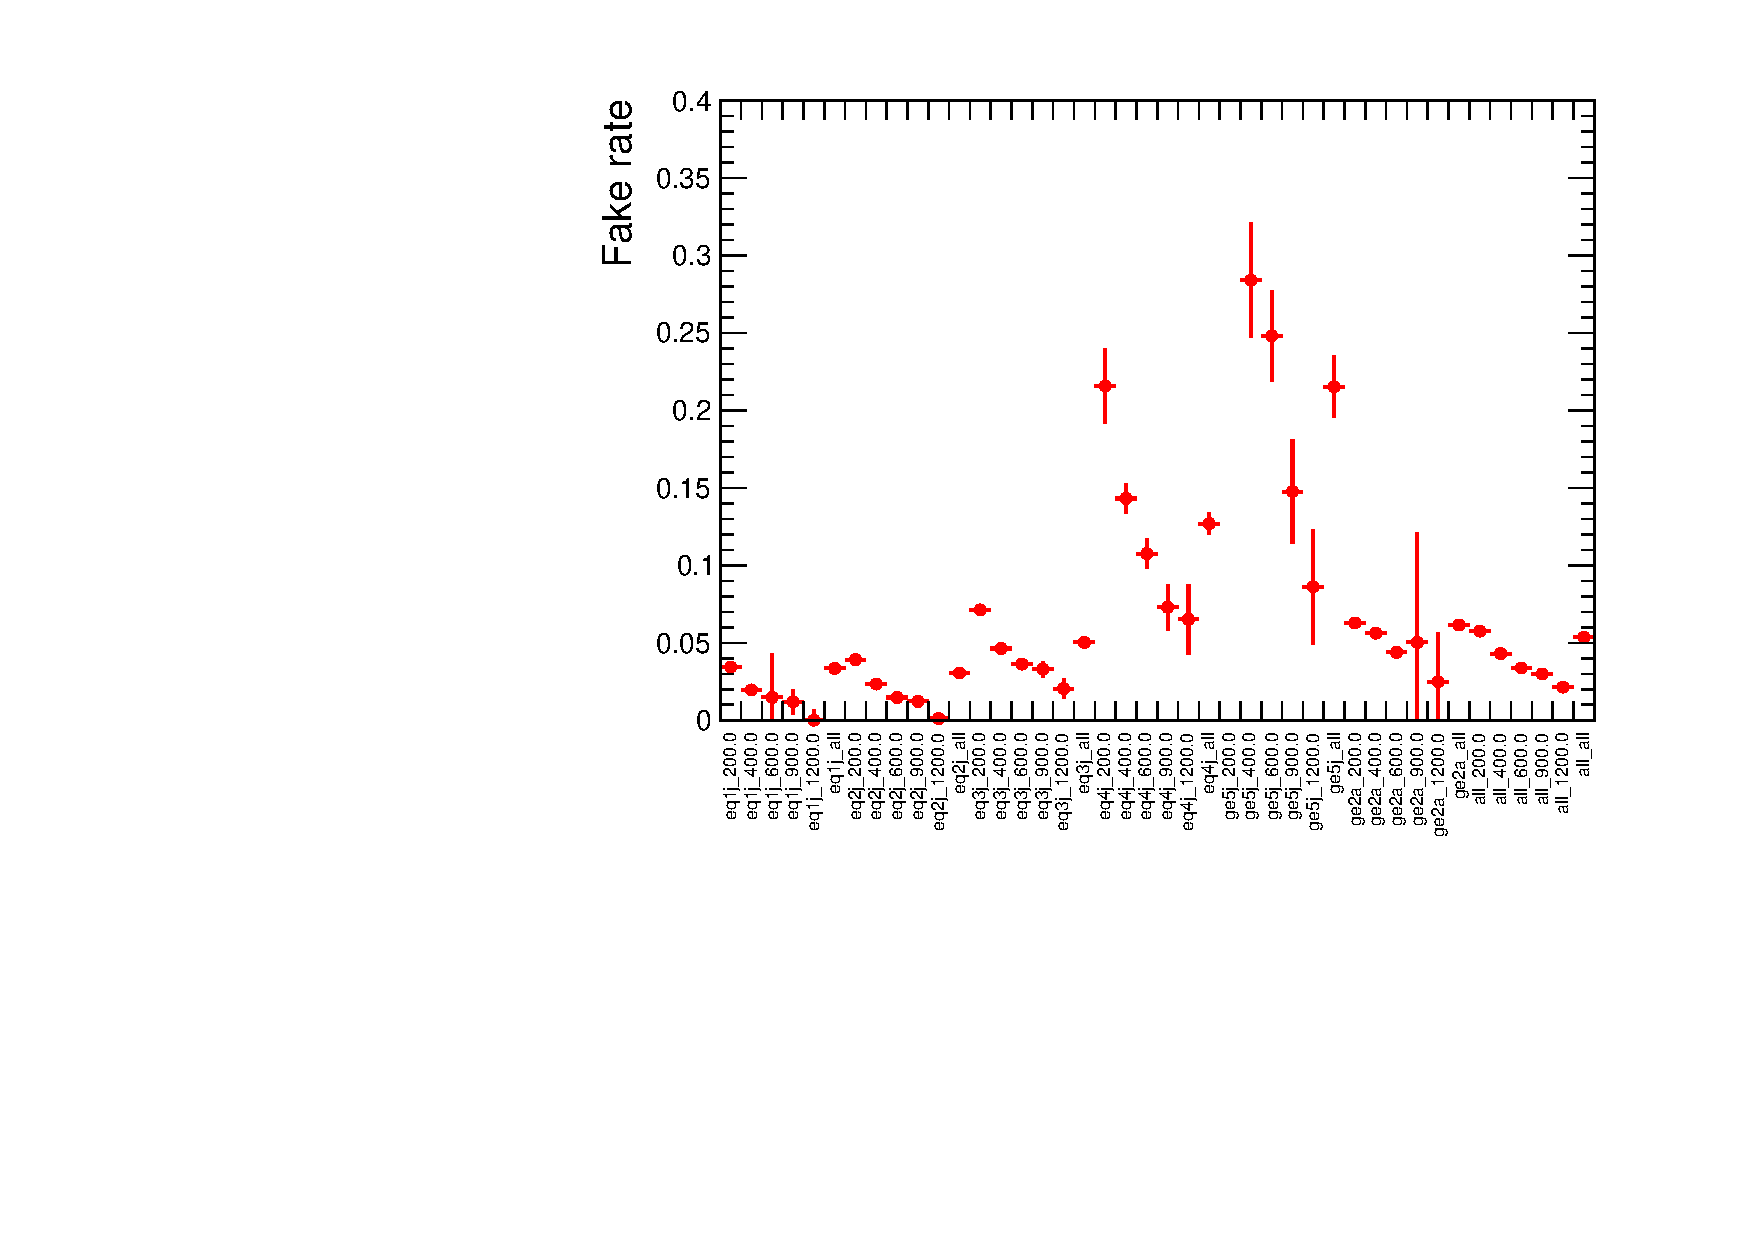
\includegraphics[width=0.45\textwidth]{figures/photonpurity/fake_rate_MC}
  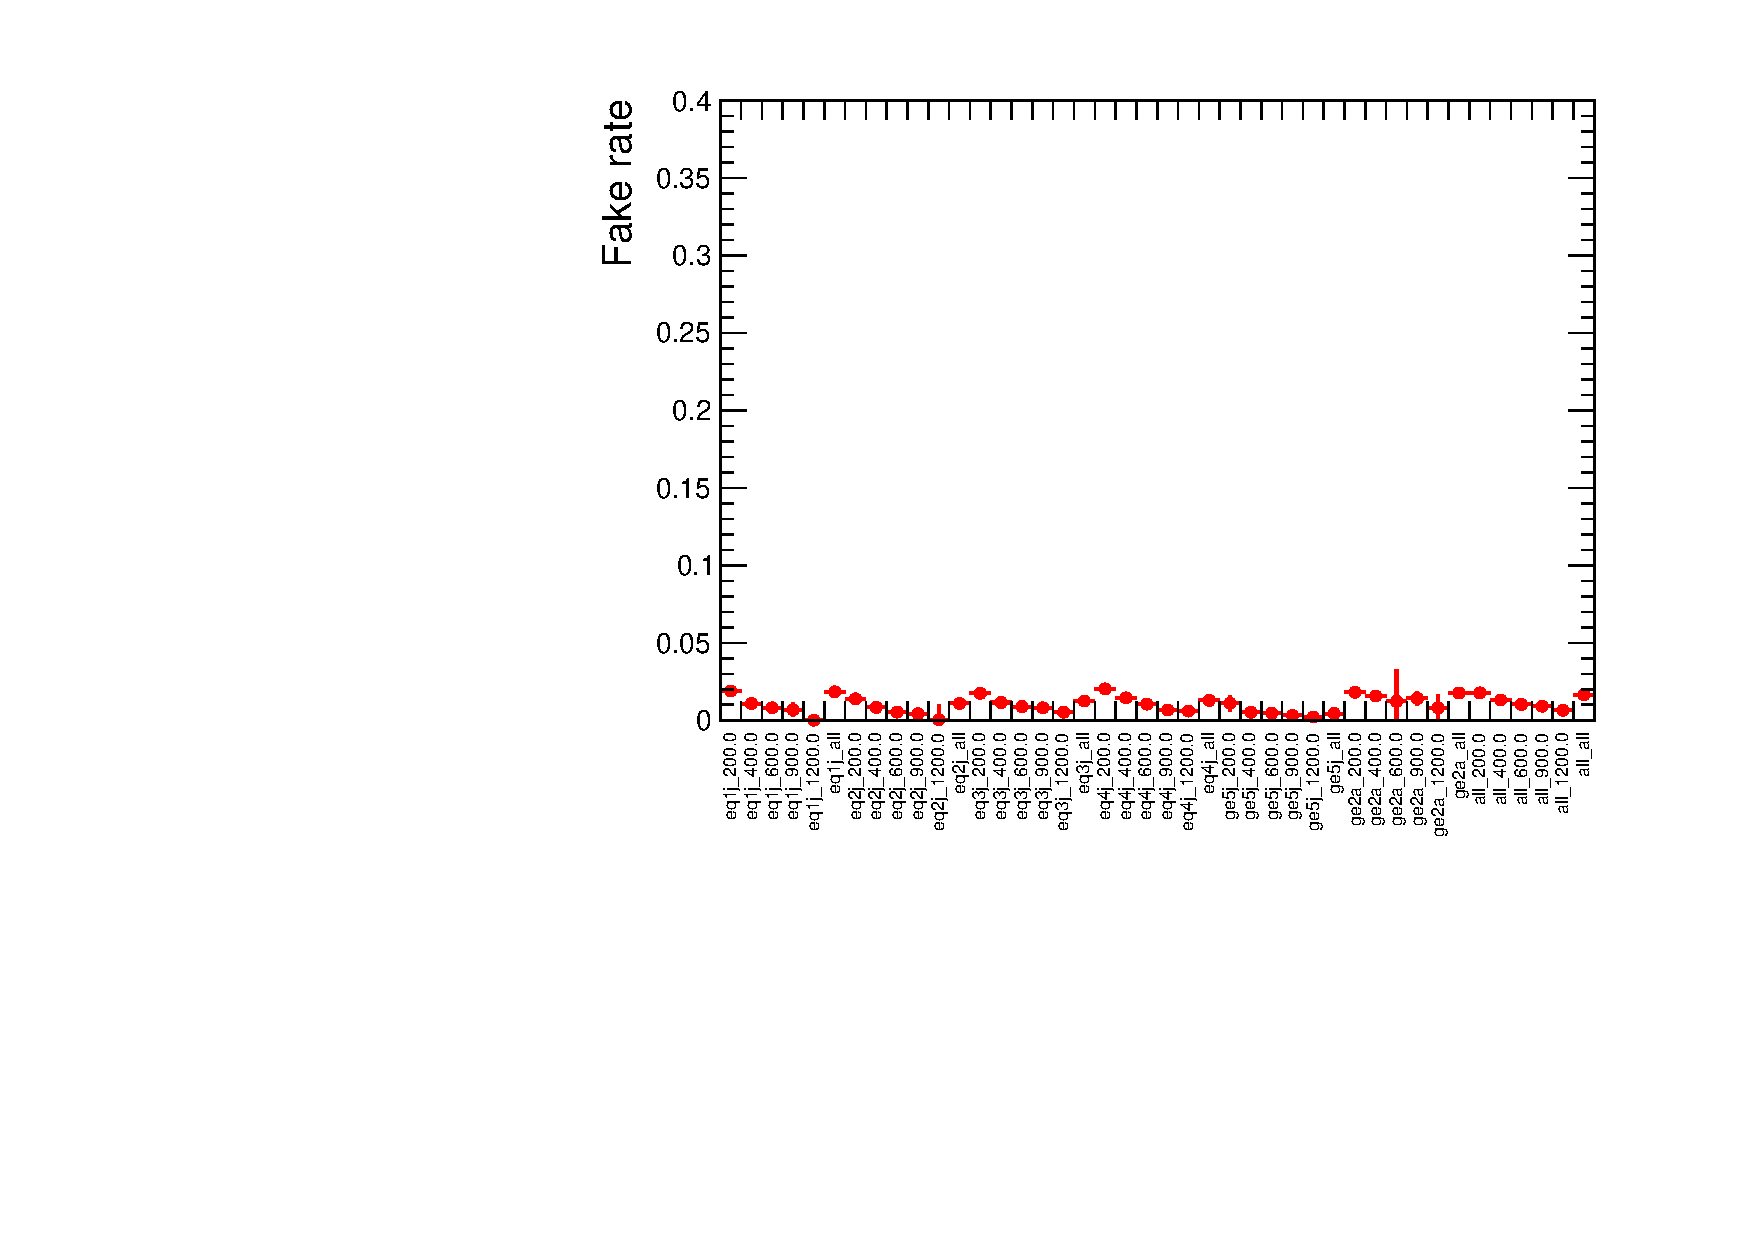
\includegraphics[width=0.45\textwidth]{figures/photonpurity/fake_rate_see}
  \caption{\label{fig:photon-purities} 
  The relative contribution of non-prompt photon as a function
  of (\njet,\HT), when using fakes templates from simulation (left)
  and from the $\sigma_{i\eta i\eta}$ sideband.}
\end{figure}


\subsubsection{Correction to \texorpdfstring{\gj}{photon+jets} cross section}
\label{sec:gj-kfactor}

The \gj cross section used in this analysis is calculated at leading
order, unlike other processes like \ttj (next-to-next-to leading
order) or \zj and \wj (next-to leading order).  A data-driven
procedure is developed to derive a ``k-factor'' for the \gj cross
section by comparing the yields in the \gj and \mmj control regions.
An inclusive correction of 1.39 is derived from the ratio of the event
yields in the two control regions and is applied to the \gj MC sample.

In order to assess the uncertainty on this correction, the systematic
sources affecting the acceptance in the \mmj control region are varied
and the effect on the event yields is derived.  They include lepton
trigger, ID, isolation, tracking efficiency and jet energy
corrections.  The total systematic uncertainty, obtained by summing in
quadrature each independent variation, is 4\% and it's propagated to
the likelihood fit.  Residual discrepancy in the $Z/\gamma$ ratio as a
function of \scalht and \njet are assessed through the data-driven
test described in Sec.~\ref{sec:closure-tests}.

\subsection{Data counts in the \texorpdfstring{\gj}{gamma+jets} control region}

\begin{figure}[h!]
  \begin{center}
    {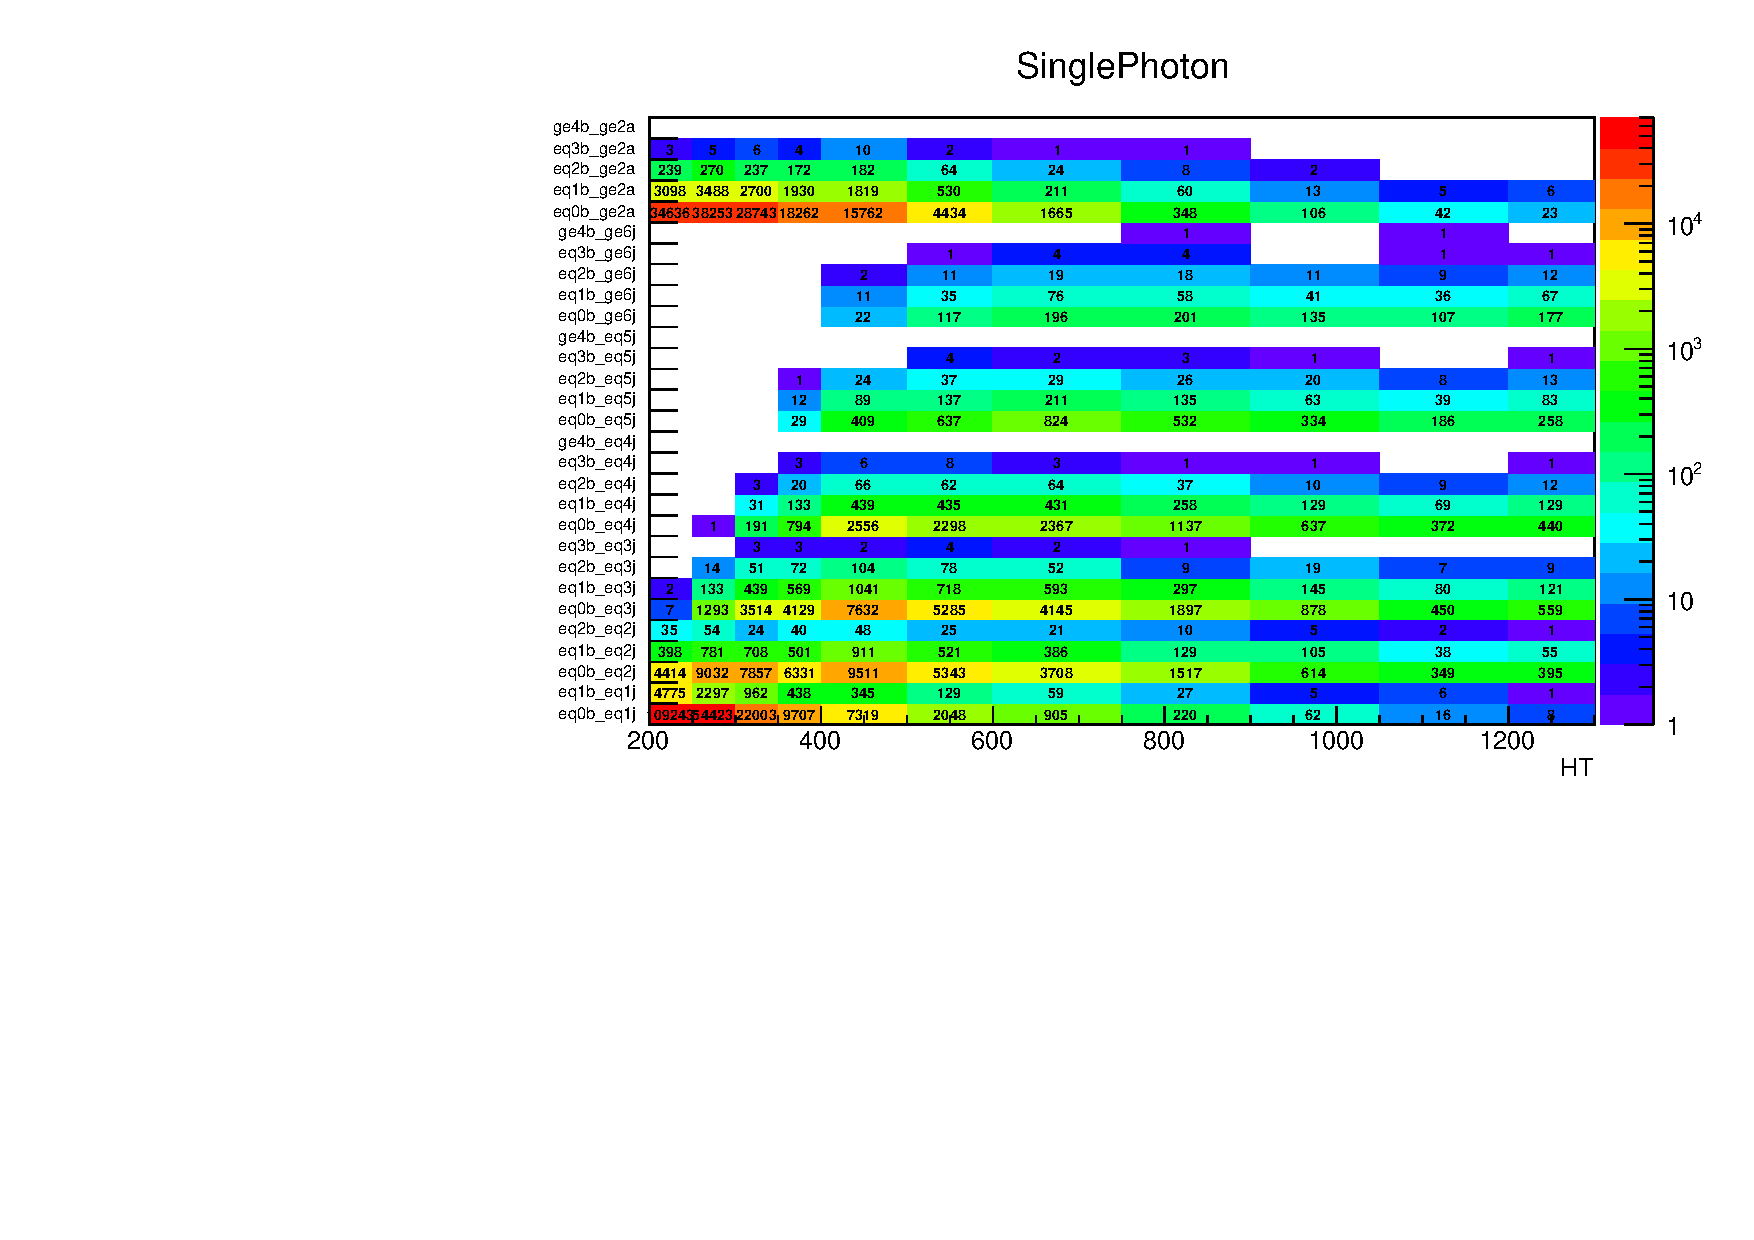
\includegraphics[width=0.6\textwidth]{figures/control_regions/SinglePhoton.pdf}}
    \caption{Event counts in data as a function of (\njet, \nb,
      \scalht) in the \gj samples. Based on 35.9\fbinv. Only event
      counts in the \mj and \mmj samples are considered when
      determining the binning utilised by the analysis. }
    \label{fig:cr-counts-gj}
  \end{center}
\end{figure}

